\documentclass[11pt,a4paper]{report}

\usepackage{amssymb,amsmath,epsfig,float,subfig,hyperref,multicol}

\usepackage{xcolor}

\definecolor{SCSUred}{HTML}{CD1041}

\hypersetup{colorlinks=true,linkcolor=SCSUred,urlcolor=SCSUred}

\usepackage{enumerate}
\usepackage{tikz}
\usetikzlibrary{arrows}
\usetikzlibrary{patterns}
\usetikzlibrary{decorations}
%%\usetikzlibrary{intersections}
\usetikzlibrary{matrix}
\usetikzlibrary{snakes}
\usetikzlibrary{calc}
\usetikzlibrary{backgrounds}

\definecolor{linecolor}{HTML}{0074C8}
\definecolor{linecolor2}{HTML}{C80200}

\newcommand{\imagebullet}[1]{\includegraphics[width=0.5cm]{#1}}

\pagestyle{empty}
\setlength{\textwidth}{7in}
\setlength{\textheight}{10in}
\setlength{\oddsidemargin}{-25pt}
\setlength{\evensidemargin}{-25pt}
\setlength{\topmargin}{-50pt}

\usepackage[english]{babel}
\usepackage[utf8]{inputenc}
\usepackage{fancyhdr}
 
%%\pagestyle{fancy}
\renewcommand{\headrulewidth}{0pt}
%%\fancyhf{}
%%\rhead{Share\LaTeX}
%%\lhead{Guides and tutorials}
%%\cfoot{OVER}

\newcommand{\DueA}{Friday, September 27}
\newcommand{\DueB}{Friday, September 27}
\newcommand{\DueC}{Monday, October 7}

\begin{document}


\begin{figure}[ht]
\begin{flushright}
	\includegraphics[width=2.0in]{U_PriHorz_WhtLtBG.jpg}
	\end{flushright}
\end{figure}

\vspace{-12mm}

\begin{flushleft}
\Large\bf \href{https://activecalculus.org/single/sec-2-1-elem-rules.html}{2.1 - Elementary Derivative Rules}\rm
%%Daily Preparation - \DueA \rm
\end{flushleft}


\vspace{8pt}

\noindent {\Large\bf{Overview}} \\
Having now completed Chapter 1 on the definition and meaning of the derivative, we turn to Chapter 2 where our principal focus will be on {\it{computing}} derivatives. By this we mean that we want to further understand the limit definition of the derivative and patterns that can be found in certain classes of functions, patterns that will enable us to {\it{simply look at the formula for a function and then be able to write down a formula for the derivative}}. As we progress through Chapter 2, you'll see that we will build from the simplest functions to much more complicated ones.\\

\noindent This section covers the following concepts: Notations for derivatives. The Power Rule. Differentiation of exponential functions. The derivative of constant multiples, sums, and differences of functions.

%%This section covers the following concept: Linearization of a function.





\vspace{16pt}

%%\pagebreak

\noindent {\Large\bf{To prepare for class}} \\
Complete all actions listed below.  Respond to the questions highlighted with {\color{SCSUred}{\boxed{Submit}}}.  %% by the start of class on {\bf{\DueA}}.  A single .pdf should be uploaded to D2L Brightspace.
\begin{itemize} \itemsep -2pt % Reduce space between items
\item {\bf{Read}} motivating questions and the introduction to \href{https://activecalculus.org/single/sec-2-1-elem-rules.html}{section 2.1} (up until Preview Activity 2.1.1).
\item[{\color{SCSUred} \boxed{Submit}}] {\bf{Do}} the following the activity that is {\it{similar}} to \href{https://activecalculus.org/single/sec-2-1-elem-rules.html#PZN}{Preview Activity 2.1.1}. 

{\bf{New Activity 2.1.1}} Start by loading the applet \href{https://www.geogebra.org/m/qwdxbtGF}{https://www.geogebra.org/m/qwdxbtGF}. Functions of the form $f(x) = x^n$, where $n = 1, 2, 3, \hdots$ are called {\it{power functions}}. The first two questions below revisit work we did earlier in Chapter 1, and the following questions extend those ideas to higher powers of $x$.
\begin{enumerate}[(a)]
\item Use the applet to determine the derivative, both the graph and a formula, of $f(x) = x^2$.  
\item Repeat part (a) for $f(x) = x^3$.  
\item Repeat part (a) for $f(x) = x^4$.  
\item Based on your work in (a), (b), and (c), what do you conjecture is the derivative of $f(x) = x^5$?  Of $f(x)= x^{13}$?
\item Make a conjecture regarding a formula for the derivative of $f(x)=x^n$ that holds for every positive integer $n$.  That is, given $f(x) = x^n$ where $n$ is a positive integer, what do you think is a formula for $f'(x)$?  
\end{enumerate}

\item[{\color{SCSUred} \boxed{Submit}}] {\bf{Extend your conjecture}} in part (d) of New Activity 2.1.1 to negative powers $n$.  That is, using $n = -1, -2, -3, \hdots$, do you spot a pattern for a formula representing $f'(x)$ if $f(x) = x^n$?  
 
\item {\bf{Watch}} the video: \href{https://www.youtube.com/watch?v=wFOgWzI0SuQ&feature=emb_title}{Quick Review: Elementary Derivative Rules (3:32)}.

\item[\imagebullet{CopilotLogo.jpg}] Prompt {\bf{Copilot}} ``What is the Binomial Theorem and how can it be used to prove the power rule in calculus for positive integers $n$?"  

\item {\bf{Do}} the following construction in \href{https://www.geogebra.org/classic?lang=en}{\it{GeoGebra}} (Google search ``GeoGebra Classic'' to use this tool if the link fails.).   Submit screenshots and responses to the questions posed. 
\begin{itemize}
\item Create a variable $a$ by typing the letter $a$ in the input box on the left.
\item A slider should be created underneath.  You will want to change the minimum and maximum values to 1.1 and 5.0 by clicking on these values at the left and right of the slider.  Set your step size to 0.01.
\item In the next input box, type $a^x$.  You will need to use the \^{ } key above the 6.  The function $f(x)=a^x$ will automatically be defined, graphed, and labeled for you. 
\item In the next input box, type {\tt{A = (0,1)}}.  This wil plot and label the point $(0,1)$ on your graph.  
\item Next, you will want to use the menu.  On the fourth button (see below), choose the {\tt{Tangents}} option.  Then, click on point {\tt{A}} on your graph followed by clicking on the graph itself.  This will produce a tangent line to your function $f(x) = a^x$ at $(0,1)$.  It will name this tangent line $g$ and an expression for it will appear in the next input box.  
\begin{figure}[H]
\begin{center}
	\includegraphics[width=2.0in]{TangentsGeoGebra.jpg}
	\end{center}
\end{figure}
\item Move the slider for $a$ as you wish by moving the big black point back and forth.  Note how your function and your tangent line change automatically!  
\item Type {\tt{ln(a)}} in the next open input box.  Move the slider and compare the slope of $g$ to this value.  What do you notice?  Does this surprise you or not?  Explain.  
\end{itemize}

\item[\imagebullet{CopilotLogo.jpg}] Prompt {\bf{Copilot}} ``Can you explain why the derivative of an exponential function is a multiple of an exponential function?"
 
\item {\bf{Read}} \href{https://activecalculus.org/single/sec-2-1-elem-rules.html#yDQ}{sections 2.1.1 and 2.1.2}.  
\item {\bf{Watch}} the video \href{https://www.youtube.com/watch?v=ciBNzth33Fw&feature=emb_title}{Derivatives of Power and Constant Functions (5:18)}.  

\item {\bf{Watch}} the video \href{https://www.youtube.com/watch?v=kcQieXhoAqs&feature=emb_title}{Derivatives of Exponential Functions (2:53)}.

%%\item {\bf{Do}} Activity 2.1.2.  


\item[{\color{SCSUred} \boxed{Submit}}]  {\bf{Complete}} \href{https://activecalculus.org/single/sec-2-1-elem-rules.html#QSl}{Exercises 1-4 in section 2.1}.  Submit four screen captures to demonstrate your completion of these four exercises. 



 

\end{itemize}

%%\pagebreak

\vspace{16pt}

\noindent {\Large\bf{After class}}\\
Solidifying the concepts discussed in class through practice is necessary to build your skills. 

%%\noindent {\large\bf{After \DueA}}
\begin{itemize}\itemsep -2pt % Reduce space between items
\item {\bf{Watch}} the video \href{https://www.youtube.com/watch?v=gya8IngB1BI&feature=emb_title}{Derivatives of Constant Multiples (4:05)}.

\item {\bf{Explore}} the concept of derivative of polynomial functions.  This \href{http://webspace.ship.edu/msrenault/GeoGebraCalculus/derivative_power_rule.html}{applet on polynomials and derivatives}, has a slider that will show the $d$th derivative of a 6th degree polynomial.  

\item {\bf{Do}} these problems.
\begin{enumerate}
\item The graph of $y = x^3-9x^2-16x+1$ has a slope of 5 at two points.  Find the coordinates of the points.  

\item 
\begin{enumerate}
\item Find the equation of the tangent line to $f(x) = x^3$ at the point where $x=2$.  
\item Graph the tangent line and the function on the same axes.  If the tangent line is used to estimate values of the function, will the estimates be overestimates or underestimates? 
\end{enumerate}

 \begin{figure}[H]
\flushright
{
  \begin{tikzpicture}[thick,scale=0.75] [domain=-3:3]
\draw[step=1cm,color=gray!30] (-4,-4) grid (4,4);
   \draw [black!80,line width=0.3pt,-latex] (0,0) -- (4,0) node [below] at (3.5,0) {$x$};
   \draw [black!80,line width=0.3pt,-latex] (0,0) -- (-4,0);
   \draw [black!80,line width=0.3pt,-latex] (0,0) -- (0,4) node [right] at (0,3.5) {$y$};
   \draw [black!80,line width=0.3pt,-latex] (0,0) -- (0,-4);
\draw[color=linecolor, line width=1.5pt,domain=-3.35:3.35]   plot (\x,0.1*\x*\x*\x);
%%  node[above] at (2,1) {$f(3,y)$};
\foreach \x/\xtext in {-4/-4, -3/-3, -2/-2,-1/-1, 1/1, 2/2, 3/3, 4/4}
    \draw[shift={(\x,0)}] (0pt,3pt) -- (0pt,-3pt) node[below] {$\xtext$};
\foreach \y/\ytext in {-4/-40,-2/-20, 2/20, 4/40}
    \draw[shift={(0,\y)}] (-2pt,0pt) -- (2pt,0pt) node[left] {$\ytext$};
\end{tikzpicture}}  
\end{figure}






\end{enumerate}
  
%%\item {\bf{Do}} Activity 2.1.3.  
\item {\bf{Do}}  \href{https://activecalculus.org/single/sec-2-1-elem-rules.html#eta}{Exercises 5-9, 11 in section 2.1}. 
 


%%\end{itemize}

%%\noindent {\large\bf{After \DueB}}
%%\begin{itemize}\itemsep -2pt % Reduce space between items
%%\item {\bf{Finish}} any in-class activities you might not have finished during class.
\item {\bf{Do}}  \href{https://activecalculus.org/single/sec-2-1-elem-rules.html#jcT}{written exercises 10, 12 in section 2.1}.  
  
\item {\bf{Start working}} on the \href{https://www.myopenmath.com/index.php}{MOMwork} (MyOpenMath) assignment for this section.  %%This will be due on \DueC.  
\end{itemize}

 
%%\pagebreak

\vspace{16pt}

\noindent {\Huge\bf{Extra Prep}}

\vspace{16pt}

\noindent {\Large\bf{Basic learning objectives}}\\
These are the tasks you should be able to perform with reasonable
fluency when you arrive at our next class meeting. Important new
vocabulary words are indicated {\it{in italics}}.  Check each box when you feel confident you have a firm grasp on that objective.  

\begin{itemize} \itemsep -2pt % Reduce space between items
\renewcommand{\labelitemi}{\scriptsize$\square$}
\item Use Leibniz notation for derivatives: $\displaystyle \frac{dy}{dx}$ as well as $\displaystyle \frac{d}{dx}$.
\item Use elementary differentiation rules to differentiate polynomials, power functions, and exponential functions.
\item Use the constant rule and the sum and difference rule to differentiate combinations of the above functions.
\end{itemize}




\vspace{16pt}

\noindent {\Large\bf{Advanced learning objectives}}\\
In addition to mastering the basic objectives, here are the tasks you should be able to perform after class, with practice:
\begin{itemize} \itemsep -2pt % Reduce space between items
\renewcommand{\labelitemi}{\scriptsize$\square$}
\item Use combinations of the rules introduced in this section to differentiate functions that are not given as a formula.
\end{itemize}

\vspace{16pt}

\noindent {\Large\bf{Need More Help?}}

\begin{itemize}\itemsep -2pt % Reduce space between items
\item {\bf{Watch}} the video: \href{https://www.youtube.com/watch?time_continue=232&v=S1fDdfX14fI&feature=emb_title}{Simplifying Before Differentiating (5:00)}. 
\end{itemize}
 
 
  \vspace{16pt}

 \noindent {\Large\bf{Selected Answers}}
\begin{enumerate}
\setcounter{enumi}{0}

\item $\displaystyle \frac{dy}{dx} = 3x^2 - 18x -16$.  So, the slope is 5 when $ 3x^2 - 18x -16=5$ or $3x^2 - 18x - 21=0$ . Solving $x^2 - 6x-7=0$ or $(x-7)(x+1)=0$ gives $x=7$ or $x=-1$.  The coordinates of these two points are thus $(-1,7)$ and $(7,-209)$.   

\item 
\begin{enumerate}
\item $f'(x)=3x^2$.  So, $f'(2)=12$.  The equation of the tangent line is $y=12x-16$.  
\item The estimates will be underestimates (since the tangent line lies below $f(x)$).  
 \begin{figure}[H]
\flushleft
{
  \begin{tikzpicture}[thick,scale=0.5] [domain=-3:3]
\draw[step=1cm,color=gray!30] (-4,-4) grid (4,4);
   \draw [black!80,line width=0.3pt,-latex] (0,0) -- (4,0) node [below] at (3.5,0) {$x$};
   \draw [black!80,line width=0.3pt,-latex] (0,0) -- (-4,0);
   \draw [black!80,line width=0.3pt,-latex] (0,0) -- (0,4) node [right] at (0,3.5) {$y$};
   \draw [black!80,line width=0.3pt,-latex] (0,0) -- (0,-4);
\draw[color=linecolor, line width=1.5pt,domain=-3.35:3.35]   plot (\x,0.1*\x*\x*\x);
\draw[color=red, line width=1.5pt,domain=-2:3.35]   plot (\x,{0.1*(12*\x-16)});
%%  node[above] at (2,1) {$f(3,y)$};
\foreach \x/\xtext in {-4/-4, -3/-3, -2/-2,-1/-1, 1/1, 2/2, 3/3, 4/4}
    \draw[shift={(\x,0)}] (0pt,3pt) -- (0pt,-3pt) node[below] {$\xtext$};
\foreach \y/\ytext in {-4/-40,-2/-20, 2/20, 4/40}
    \draw[shift={(0,\y)}] (-2pt,0pt) -- (2pt,0pt) node[left] {$\ytext$};
\end{tikzpicture}}  
\end{figure}
\end{enumerate}





\end{enumerate}


\end{document}

